% ****** Start of file apssamp.tex ******
%
%   This file is part of the APS files in the REVTeX 4.1 distribution.
%   Version 4.1r of REVTeX, August 2010
%
%   Copyright (c) 2009, 2010 The American Physical Society.
%
%   See the REVTeX 4 README file for restrictions and more information.
%
% TeX'ing this file requires that you have AMS-LaTeX 2.0 installed
% as well as the rest of the prerequisites for REVTeX 4.1
%
% See the REVTeX 4 README file
% It also requires running BibTeX. The commands are as follows:
%
%  1)  latex apssamp.tex
%  2)  bibtex apssamp
%  3)  latex apssamp.tex
%  4)  latex apssamp.tex
%
\documentclass[%
%superscriptaddress,
%groupedaddress,
%unsortedaddress,
%runinaddress,
%frontmatterverbose, 
%preprint,
%showpacs,preprintnumbers,
%nofootinbib,
%nobibnotes,
%bibnotes,
 amsmath,amssymb,
 aps,
 twocolumn,
 prl,
 reprint,
%pra,
%prb,
%rmp,
%prstab,
%prstper,
floatfix,
]{revtex4-1}

\usepackage{graphicx}% Include figure files
\usepackage{dcolumn}% Align table columns on decimal point
\usepackage{bm}% bold math
\usepackage{lineno}
\usepackage{color}
\usepackage{acronym}
%\addbibresource{references.bib}
\linenumbers % Commence numbering lines
%\usepackage{hyperref}% add hypertext capabilities
%\usepackage[mathlines]{lineno}% Enable numbering of text and display math
%\linenumbers\relax % Commence numbering lines

%\usepackage[showframe,%Uncomment any one of the following lines to test 
%%scale=0.7, marginratio={1:1, 2:3}, ignoreall,% default settings
%%text={7in,10in},centering,
%%margin=1.5in,
%%total={6.5in,8.75in}, top=1.2in, left=0.9in, includefoot,
%%height=10in,a5paper,hmargin={3cm,0.8in},
%]{geometry}

%% ----- some handy shortcuts
\newcommand{\dcc}{LIGO-PXXXXXXXX}

\newcommand{\chris}[1]{\textbf{\textcolor{green}{CHRIS: #1}}}

%% ----- input git-version tag
\input{tag.tex}

\begin{document}

\preprint{APS/123-QED}

%
% Be clear and specific. Do not claim too much or too little.
%
\title{Matching Matched Filtering with Deep Networks in Gravitational wave Astronomy}

\author{Hunter Gabbard}
 \email{Corresponding author: h.gabbard.1@research.gla.ac.uk}
\author{Fergus Hayes}
\author{Chris Messenger}
\author{Michael Williams}
\affiliation{
 SUPA, School of Physics and Astronomy, \\
 University of Glasgow, \\
 Glasgow G12 8QQ, United Kingdom \\
}

%\date{\today}% It is always \today, today,
             %  but any date may be explicitly specified

\date{\commitDATE\\\mbox{\small \commitID}\\\mbox{\dcc}}

%
% Explain what the result is and why it’s important, plus possibly a sentence
% or two of introduction, motivation, methods, caveats.
%
\begin{abstract} 
%
We reprt on the construction of a deep convoloutional neural network that can
achieve the same  
We report a new method for classifying gravitational-wave (GW)
signals from binary black hole (BBH) mergers using a deep convolutional neural
network. Using only the raw time series as an input, we are able to distinguish
GW signals injected in Gaussian noise amongst instances of purely Gaussian
noise time series with (\textbf{need figure of merit here}) percent accuracy.
We compare our results with the standard method of matched filtering used in
Advanced LIGO and find the methods to be comparable.  
\begin{description}
\item[PACS numbers] May be entered using the \verb+\pacs{#1}+ command.
\end{description} 
%
\end{abstract}

\pacs{Valid PACS appear here}% PACS, the Physics and Astronomy
                             % Classification Scheme.
%\keywords{Suggested keywords}%Use showkeys class option if keyword
                              %display desired


\maketitle

\acrodef{GW}[GW]{gravitational-wave}
\acrodef{BBH}[BBH]{binary black hole}
\acrodef{SNR}[SNR]{signal-to-noise ratio}
\acrodef{GPU}[GPU]{graphics processing unit}
\acrodef{PSD}[PSD]{power spectral density}
\acrodef{BNS}[BNS]{binary neutron star}
\acrodef{FFT}[FFT]{fast Fourier transform}

%\tableofcontents

%
% Explain what the result is and why it’s important, particularly arguing how
% the paper will move physics forward. Like the abstract, but shorter and with
% a focus on WHY not HOW.
%

%
% Give sufficient background so the general reader can understand what you did
% and why you did it.
%
\textit{Introduction} --- 
%
% intro to gravitational waves
%
The field of gravitational wave astronomy has seen an explosion of compact
binary coalescence detections over the past several years. The first of these
were binary black hole detections~\cite{PhysRevLett.116.061102,
PhysRevLett.116.241103, PhysRevLett.118.221101} and more recently the advanced
detector network made the first detection of a binary neutron star
system~\cite{PhysRevLett.119.161101} seen in conjuction with a gamma-ray
burst~\cite{2017arXiv171005834L,2017arXiv171005446G,2017arXiv171005449S} and
multiple post-merger electromagnetic signatures~\cite{2017arXiv171005833L}.
These detections were made possible by the Advanced Laser Interferometer
Gravitational wave Observatory (aLIGO) detectors, as well as the recent joint
detection of GW170814 with Advanced Virgo \cite{PhysRevLett.119.141101}. Over
the coming years many more such observations, including \ac{BBH} and binary
neutron stars but also other more exotic sources such as intermediate black
holes (IMBH), and neutron star black hole (NSBH) mergers, are likely to be
observed on a more frequent basis. As such, the need for more efficient search
methods will be more pertinent as the detectors increase in sensitivity.

%
% describe the existing algorithms
%
The algorithms used to make these detections \cite{0264-9381-33-21-215004}
[\textbf{cite gstlal too??}]~\chris{yes!} are computationally expensive to run.
Part of the reason being that the methods used by these \textit{search
pipelines} are complex, sophisticated processes run over a large parameter
space using advanced signal processing techniques. Distinguishing noise from
signal in this search pipeline, and others like it, is done using a technique
called matched template filtering~\chris{not template based matched
filtering?}. 

%
% introduce matched filtering
%
Matched template filtering uses a \textit{bank} of template waveforms that span
the astrophysical parameter space \cite{PhysRevD.44.3819, PhysRevD.49.1707,
PhysRevD.53.6749, PhysRevD.60.022002, 0264-9381-23-18-002, PhysRevD.80.104014,
PhysRevD.86.084017, PhysRevD.89.084041, PhysRevD.87.124003, 1307.4158,
PhysRevD.89.024003, PhysRevD.93.124007}~\chris{might be a few too many
references for template banks here. What about waveform references?}. A
template bank will span a large astrophysical parameter space since we do not
know \textit{a priori} what the true parameters of the gravitational waves will
be. The waveforms of the signals are well modeled by post-Newtonian
theiry~\cite{PhysRevD.84.049901,PhysRevD.80.084043,Blanchet2014,PhysRevD.93.084054},
and analysis pipelines use matched filtering to search for those signals buried
in the detector noise. More on how we implement this technique and further
comparisons with our model will be described later in this letter.

%
% introduce deep learning
%
Deep learning is a subset of machine learning which has gained in popularity in
recent years~\cite{NIPS2012_4824, 1406.2661, 1409.1556, 1412.7062, 1311.2901,
1409.4842} with the rapid development of \ac{GPU} technology. Some successful
implementations of deep learning have been used in the colorization of black
and white images \cite{1603.08511}, automatic image caption generation
\cite{1412.2306}, object classification and detection in photographs
\cite{NIPS2012_4824}, along with many other exciting applications~\chris{this
is a bit photograph heavy, can we find some scientific applications, e.g.,
medical, bio-science, etc.. }. One advantage of deep learning is its ability to
perform analyses very rapidly since the method's computationally intensive
stage is pre-computed during the training step prior to the analysis of actual
data. This results in low-latency searches that are several orders of magnitude
faster~\cite{726791} than other comparable classification methods. 

%
% more detail on deep learning
%
A deep learning algorithm is composed of arrays of processing units, called
neurons, which can be anywhere from one to several layers deep. A neuron acts
as a filter, whereby it is passed a vector of inputs, performs a transformation
on them and then outputs a single scalar value. Deep learning algorithms
typically consist of an input layer, followed by one to several hidden layers
and then one to $N$~\chris{what is $N$? Don't introduce something without
defining it or that we won't use again.} fully-connected neurons. This value
can then either be used to solve classfication, or regression-like problems. In
the case of classification, each output neuron corresponds to the probability
that a particular input sample is of a certain class.

%
% what are we going to do
%
In this letter we investigate the simplest case of establishing whether a
signal is present in the data or if the data contains only detector noise. We
propose a deep learning procedure requiring only the raw data time
series as input with minimum signal pre-processing. We show how this approach
can be pre-trained using simulated data-sets and applied in low-latency 
to acheive the same sensitivity as established matched filtering techniques. 

%
% the structure of the paper
% 
In the following sections we will discuss our choice of network architecture
and tuning of it's hyperparameters, compare the results of our network with the
widely used matched-filtering gravitational-wave signal classification
technique, and comment on future improvements and applications of this work.      

%
% Try to be clear, e.g. use heuristic explanations. But making a strong case
% for the result takes precedence. You can submit Supplementary Material or,
% better, an accompanying longer paper.
%
\textit{Simulation details} --- 
%
% describe the simulations
%
In order to make a clean comparison between a deep learning approach and
matched-filtering, we distinguish between only 2 cases, \ac{BBH} merger signals
in additive Gaussian noise (signal+noise) and Gaussian noise alone
(noise-only). We choose to focus on \ac{BBH} signals only rather than including
\ac{BNS} systems for the reason that \ac{BBH} systems are higher mass systems
and have shorter duration signals once the inspiralling systems have entered
the Advanced LIGO frequency band. They typically then merge on the timescale of
$\mathcal{O}(1)$ sec allowing us to use a relatively small datasets for this
study. The input datasets consist of simulated gravitational wave timeseries
data that has been whitened in the frequency domain. This process rescales the
noise contribution at each frequency to have equal power resulting in "white"
noise. The signal (if present) has it's constituent frequency components
reweighted according to the \ac{PSD} used.    

%
% describe the noise (Gaussian)
%
Our noise is generated from a \ac{PSD} equivelent to the projected Advanced
LIGO design sensitivity. The \ac{PSD} is used to draw random complex Gaussian
amplitudes to construct frequency series to which we apply an inverse \ac{FFT}
to obtain time domain realisations representing LIGO detector noise.

%
% describe the signal generation 
%
Signals are simulated using a library of gravitational wave data analysis
routines called \texttt{LALSuite}. We use the IMRPhenomD type
waveform~\cite{PhysRevD.93.044006, PhysRevD.93.044007} which models the
inspiral, merger and ringdown components of \ac{BBH} gravitational wave
signals. We simulate systems with component black hole masses in the range from
5\(M_\odot\) to 100\(M_\odot\), $m_{1} > m_{2}$, and all with zero
spin~\chris{We ned to describe how we draw these masses}. Each
injection is given a random right ascension and declination assuming an
isotropic prior on the sky, the polarization angle and phase are drawen from a
uniform prior on the range $[0,\pi]$, and the inclination angle is drawn such
that the cosine of inclination is uniform on the range $[-1,1]$. The waveforms
are then randomly placed within the time series, see figure \ref{fig:waveform},
such that the peak of the waveform is within the final $20$\% of the time
series. The waveform amplitude is scaled to achieve a predefined optimnal
\ac{SNR} defined as
%
% the optimal SNR
%
\begin{equation} \label{eq:snr}
\rho_{\mathrm{opt}}^{2} = 4 \int_{f_{\mathrm{min}}}^{\infty} \frac{\lvert
\tilde{h(f)}\rvert^{2}}{S_{\mathrm{n}}(f)} \mathrm{d}f,
\end{equation}
%
where $\tilde{h(f)}$ is the frequency domain representation of the
gravitational wave strain,m $S_{\mathrm{n}}(f)$ is the detector noise \ac{PSD},
and $f_{\mathrm{min}}$ is the frequency at which we start to accumulate
\ac{SNR}. The simulated time series were chosen to be 1~sec in duration sampled
at 8192 Hz and therefore in our case we consider $f_{\mathrm{min}}$ as the
frequency of the gravitational wave signal at the start of the sample
timeseries. An example timeseries can be seen in Figure~\ref{fig:waveform}. 

%
% How many sampes did we make
%
Our datasets contain 50,000 independent timeseries with 50\% containing
signal+noise and 50\% noise-only. For each simulated gravitational wave signal
(drawn from the signal parameter space) we generate 25 independent noise
realisations from which 25 signal+noise samples are produced. This procedure is
standard within machine learning classification and allows the network to learn
how to identify individual signals under different noise scenarios. Each
noise-only sample consists of an independent noise realisation and in total we
use 1000 unique waveforms in the $m_{1},m_{2}$ mass space. Each data sample
timeseries is then represented in the form of a $1 \times 8192$ pixel image
with the grayscale intensity of each pixel proportional to the gravitational
wave amplitude.

%
% How we split training, validation, and testing
%
Supervised deep learning approaches to classification problems require
datasets to be sub-divided into training, validation, and testing sets.
Training sets are the data samples that the network learns from, the validation
set allows the developer to verify that the network is learning correctly, and
the test set is used to quantify the performance of the trained network.  
Of the datasest generated we use $70\%$ of these samples for training,
$15\%$ for validation, and $15\%$ for testing.

\begin{figure} 
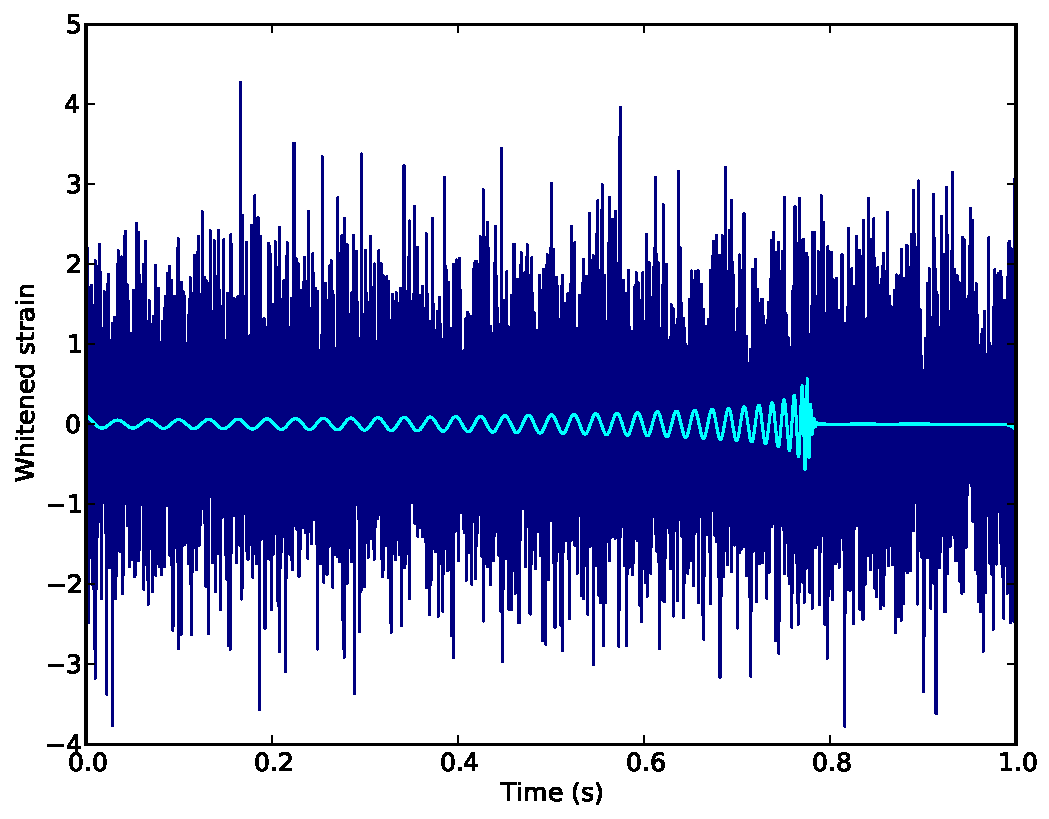
\includegraphics[width=\columnwidth]{figures/waveform.pdf}
\caption{\label{fig:waveform} The amplitude time series shown above illustrates
an injection waveform at SNR (\textbf{need value}) superimposed on a whitened
Gaussian noise time series with the injection waveform signal injected into the
noise. Sample time series such as this are then converted to a 1 $\times$ 8192
pixel image. Those images are then used as our training, validation and testing
samples.}
\end{figure}

%
% define the CNN structure 
% 
\textit{Network Structure} --- 
%
%
%
In our model, we use a variant of a deep learning algorithm called a
convolutional neural network (CNN) \cite{726791}.  CNN layers are composed of
five primary variants: input, convolutional, activation, pooling, and
fully-connected. Where input holds the raw pixel values of the sample image,
the convolutional layer computes the convolution between the kernel and a local
region of the input layer volume, activation applies an elementwise activation
function leaving the size of the previous layer's output volume unchanged,
pooling performs a downsampling operation along the spatial dimensions, and the
fully-connected layer computes the class scores using an error function,
cross-entropy, defined as

\begin{equation} \label{eq:loss}
f_{\theta^{'}}(\theta) = -\sum_{i} \theta_{i}^{'} \mathrm{log}(\theta_{i}),
\end{equation}

where $\theta_{i}$ is the predicted probability distribution of class $i$ and
$\theta_{i}$ is the true probability for that class
\cite{tensorflow2015-whitepaper}. 

In order to achieve the optimal network, multiple sets of hyperparameters are
tuned. First, we rescaled the data, but with the existing setup, this did not
seem to improve upon the performance. We also attempted applying transfer
learning where we used networks trained on successively higher SNR values,
though performance benefits were minimal. Network depth was adjusted between 2
to 10 convolutional layers. Our initial data set needed at least 4
convolutional layers. Later data sets with various noise realizations needed
fewer convolutional layers to perform comparatively well, but adding more
layers still seemed to improved performance. The inclusion of dropout was used
within the fully-connected layers as a form of regularization.

For updating our weights and bias parameters (in order to minimize our loss
function, $f(\theta)$, \eqref{eq:loss}) we settled on the nesterov momentum
optimization function

\begin{equation} \label{eq:nesterov1}
v_{i+1} = \mu v_{i} - \epsilon \nabla f(\theta_{i} + \mu v_{i}),
\end{equation}

\begin{equation} \label{eq:nesterov2}
\theta_{i+1} = \theta_{i} + v_{i+1},
\end{equation} \\

where $\epsilon > 0$ is the learning rate, $\mu \in [0,1]$ is the momentum
coefficient, and $\nabla f(\theta_{i})$ is the gradient with respect to the
weight vector $\theta_{i}$. Nesterov momentum was the ideal choice because of
its prescient ability to approximate the next position of the weights and bias
parameters which therefore gives a rough approximation of their values. Thus
the gradient is calculated not with respect to the current parameters, but with
respect to the approximate future positions of those parameters
\cite{Sutskever:2013:IIM:3042817.3043064}. A further detailed description of
the neural network architecture used can be found in Table \ref{table:network}.

\begin{figure}[!h] 
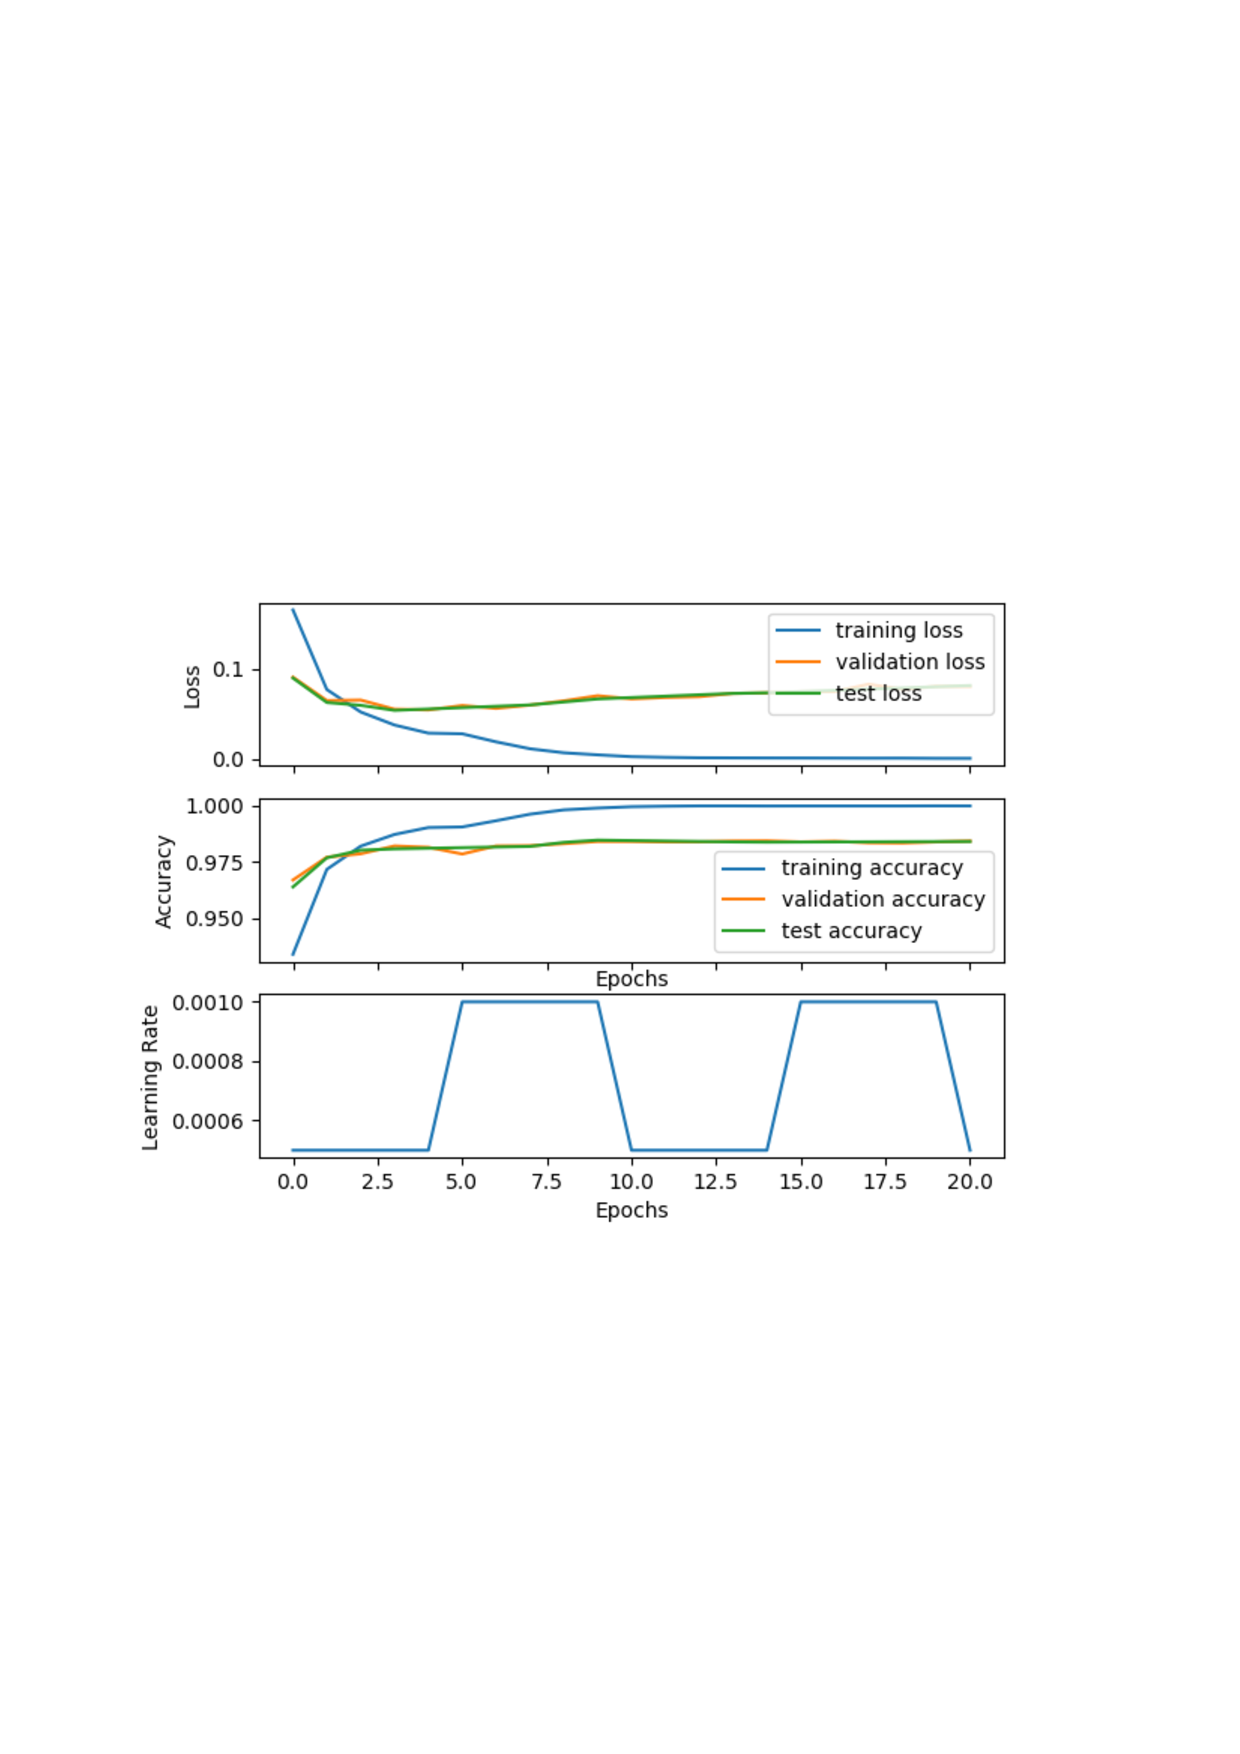
\includegraphics[width=0.5\textwidth]{figures/loss.pdf}
\caption{\label{fig:loss_curve} The loss, accuracy and learning rate plots
(shown above) illustrate how the network's performance is defined as a function
of the number of training epochs. The goal is to minimize the loss function,
which will in turn maximize the accuracy of the classifier. The first initial
epochs see an exponential decrease in the loss function and then a slowly
falling monotonic curve to follow. This indicates that the longer our network
is trained, a limit with respect to the accuracy is approached. In our case, we
cyclically adjust the learning rate to oscialte between $5 \times 10^{-4}$ and
$1 \times 10^{-3}$ at a constant frequency. Studies have shown that this policy
of learning rate adjustement (\textbf{should replace figure with better run})}
\end{figure}

Largely following matched filtering techniques used on the LIGO Open Science
Center optimal matched filter page \cite{1742-6596-610-1-012021} we compare our
results to the standard optimal matched filtering process used by aLIGO
\cite{PhysRevD.85.122006}. Considering the example of one candidate GW signal,
we iterate over a comprehensive template bank. The template bank was generated
using 8000 randomly sampled mass pairs from the same distribution with no
adjustment to assure the parameter space was adequately covered. For each
template, we compute the Fast Fourier Transform (FFT) of the data and the
template, where the template has been zero padded in order for both to be of
the same length. Finally, we multiply the fft'd template and data together and
divide by the PSD. An inverse FFT is then applied in order to convert back to
the time domain. The output is then normalized so that we have an expected
value of 1 for pure Gaussian noise.

\begin{table*}[]
\centering
\caption{The optimal network structure (seen below) was determined through
multiple tests and tunnings of hyperparameters by means of trial and error. The
network consists of 8 convolutional layers, followed by 2 fully-connected
layers. Max-pooling is performed on the first, fifth, and eigth layer, whereas
dropout is only performed on the two fully-connected layers. Each layer uses an
Elu activation function while the last layer uses a Softmax activation function
in order to normalize the output values to be between zero and one so as to
give a probability value for each class.} \label{table:network}
\begin{tabular}{lllllllllll}
                    & layer 1 & layer 2 & layer 3 & layer 4 & layer 5 & layer 6 & layer 7 & layer 8 & layer 9 & layer 10 \\
Number of Kernals   & 8       & 16      & 16      & 32      & 64      & 64      & 128     & 128     & 64      & 2        \\
Filter Size         & 32      & 16      & 16      & 16      & 8       & 8       & 4       & 4       & n/a     & n/a      \\
Max Pooling         & yes       & no       & no       & no       & yes       & no       & no       & yes       & no     & no      \\
Fully Connected     & no     & no     & no     & no     & no     & no     & no     & no     & yes     & yes      \\
Drop out            & 0.0     & 0.0     & 0.0     & 0.0     & 0.0     & 0.0     & 0.0     & 0.0     & 0.5     & 0.5      \\
Activation Function & Elu     & Elu     & Elu     & Elu     & Elu     & Elu     & Elu     & Elu     & Elu     & Softmax 
\end{tabular}
\end{table*}

\textit{Results} --- After tunning several hyperparameters and then settling on
an ideal network format (Table \ref{table:network}), we present the results of
our classifier on a noise vs. injection sample set. We trained our network
using a transfer learning approach whereby we initially trained our network on
a sample set of 1000 noise and 1000 injection signals (each with 25 different
noise realizations) with an integrated SNR value of 12. We then lowered the
integrated SNR value by 2 and (using the same weights from our previous
network) we trained our classifier again. This approach seemed to only have a
marginal benefit on the overall performance of the classifier.  

The confusion matrix in figure \ref{fig:confusion} shows $99.86\%$ accuracy
with triggers at an integrated SNR of 12, $99.64\%$ accuracy with integrated
SNR 10, $97.88\%$ at integrated SNR 8, $88.72\%$ at an integrated SNR of 6,
$68.34\%$ at integrated SNR 4, and $50.19\%$ accuracy at integrated SNR 2.


\begin{figure}[]
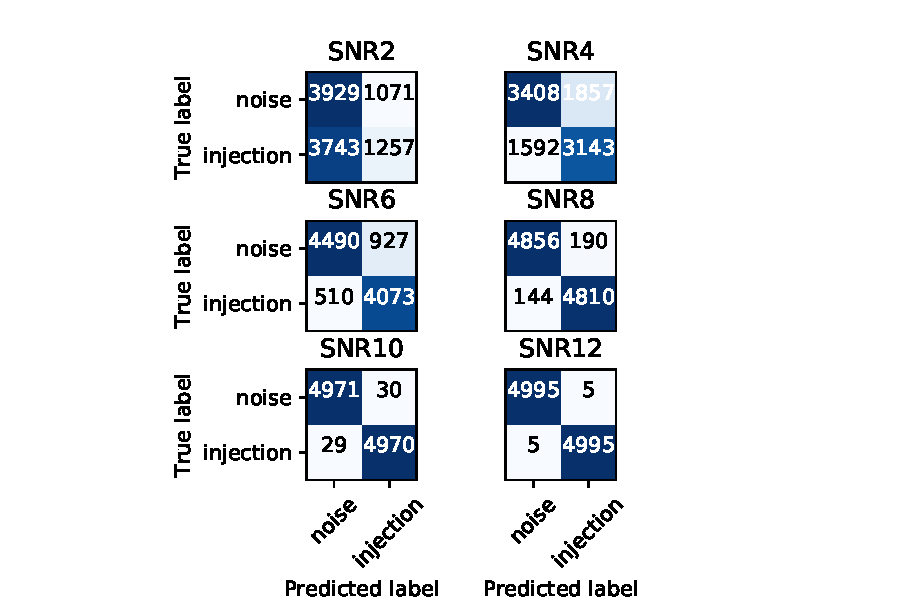
\includegraphics[width=0.5\textwidth] {figures/confusion_matrix.pdf}
\caption{\label{fig:confusion} Confusion matrices for runs from SNR 2 - SNR 12.
Numbers superimposed on bins represent the number of samples corresponding to
samples that are either true positive, true negative, false negative, or false
positive. The accuracy percentages for all injection SNR values are listed as
follows: $50.19\%$ at SNR 2, $68.34\%$ at SNR 4, $88.72\%$ at SNR 6, $97.88\%$
at SNR 8, $99.64\%$ at SNR 10 and $99.86\%$ at SNR 12.}
\end{figure}

In figure \ref{fig:ROC_curve} we compare our results to that of matched
filtering where we use two alternative match filtering methods. The first,
using the nominal template bank described in the \textit{Sample Simulation
Methods} section, whereas the second uses the optimal template for each
injection, whereby optimal is defined as the template used to generate that
injection. As seen in figure \ref{fig:ROC_curve} all three methods have
equivalent performance proficiency at $\sim \mathrm{iSNR} > 9$, whereas there
is a marginal dip in performance in the nominal matched filtering method and
our deep learning classifier. It should be noted that our classifier exceeds
the performance proficiency of that of the nominal matched filtering method
between iSNR 2 and iSNR 4. 

\begin{figure}[] 
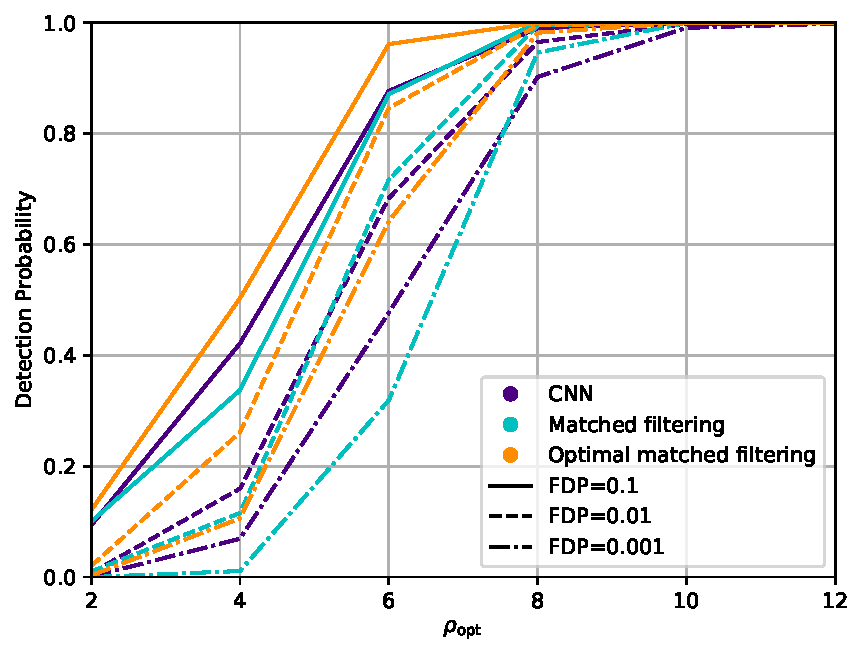
\includegraphics[width=0.5\textwidth] {figures/accuracy.pdf}
\caption{\label{fig:ROC_curve} Using a predetermined false alarm probability
value of $0.01$ we compute the receiver operating curve (ROC) plot the
detection probability as a function of the SNR. As can be seen in the plot, our
classifier performs marginally poorer than standard matched filtering at SNR
$>$ 6 and exceeds standard matched filtering at SNR $<$ 6. The matched
filtering curve using the optimal template for each injection exceeds the
performance of both the standard matched filtering and deep learning
classification methods.} 
\end{figure}

We compare the results of all three methods at various injection iSNR values in
figure \ref{fig:isnr_curves}. It is not surprising to see that the matched
filtering method using the optimal template consistantly performs better than
both the nominal match filtering method and our deep learning classifier.
However, what is considerable is the comparison between the nominal matched
filtering and the deep learning classifier detection probability curves. It can
clearly be seen that our classifier exceeds the performance of the nominal
matched filtering method at iSNR 2, 4 and 6. This is a promising result and
certainly merits further investigation.  

\begin{figure}[] 
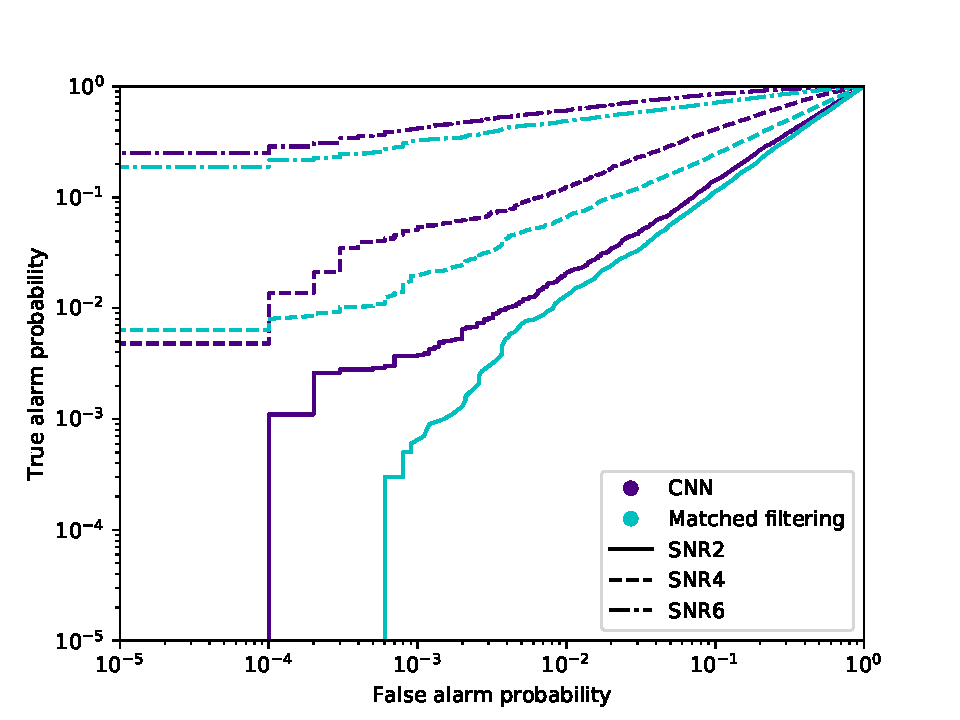
\includegraphics[width=0.5\textwidth] {figures/ROC_curves.pdf}
\caption{\label{fig:isnr_curves} Shown above are receiver operating curves for
runs using injections at SNR 2, 4, 6, 8, 10, and 12. Each figure is plots
detection probability as a function of the false detection probability rate.}
\end{figure}

%
% Summarise what you did, note key equations and specific results. If there is
% a main numerical result, quote it here. Then go back and make sure the
% abstract contains the most important results. Say what’s next
%
\textit{Conclusions} --- In conclusion, we demonstrate that deep learning, when
applied to a raw data time series, is able to produce equivalent results to
matched template filtering. We employ a deep convolutional neural network with
carefully chosen hyperparamters and produce an output that returns the class
probability value of any given signal. This output could then further be
applied as a ranking statistic in the aLIGO CBC search. Although only BBH
mergers were used, this method could also easily be applied to other merger
types, such as BNS and NSBH signals. The results shown in both figure
\ref{fig:ROC_curve} and figure \ref{fig:isnr_curves} indicate that deep
learning approaches even have the unprecedented potential to entirely exceed
matched template filtering. 

\emph{Acknowledgements}---We would like to acknowledge valuable input from the
LIGO-Virgo Collaboration specifically the machine-learning working group. The
authors also gratefully acknowledge the Science and Technology Facilities
Council of the United Kingdom.  CM is supported by the Science and Technology
Research Council (grant No.~ST/~L000946/1).
%
%\end{acknowledgments}


% The \nocite command causes all entries in a bibliography to be printed out
% whether or not they are actually referenced in the text. This is appropriate
% for the sample file to show the different styles of references, but authors
% most likely will not want to use it.

\bibliographystyle{apsrev4-1}
\bibliography{references}% Produces the bibliography via BibTeX.


\end{document}
%
% ****** End of file apssamp.tex ******
